\section{Verification and measured performance}
\label{sec:experiments}

The experiments answer four different questions: whether the mathematical
conditions agree with independent finite oracles, whether new production
certificates pass the old checkers, how much work the new local operations
save, and whether those savings survive the surrounding recognition
pipeline. These questions have different test populations and timing
boundaries. Their results must not be pooled into one speedup figure.

\subsection{Evidence and measurement protocol}

All reported measurements use Python 3.12.14 in the supplied Linux
environment. They are observations from one environment, without a claim
of dedicated hardware or machine-independent milliseconds. The archive
retains exact inputs, fixed random seeds, shuffled call orders, every
measured sample, excluded warmups, work counters, reasons for resource
exhaustion, and hashes of the source modules actually loaded. The numerical
tables and figures are generated from these records.

The group benchmarks load the pinned package and the changed package
under separate module names in one process. Each timed call constructs a
fresh diagram and search state. Three arms compare the baseline, the new
code with saturation disabled, and the new code with saturation enabled.
There is one excluded warmup and five measured rounds with shuffled
orders. The disabled arm detects effects unrelated to the new policy; the
abstract kernel also has an exactly identical ordinary-search control.
The two orbit experiments instead use seven measured rounds and identical
function controls, with their precise preparation boundaries stated below.

Elapsed times are medians of complete calls. A reported ratio is the median
of the within-round baseline/new ratios, so it need not equal the quotient
of the two displayed medians. A ratio is supplied only if all measured
pairs reach the same conclusive result. An exhausted work, node, or time
allowance is not a completion time. Its observed elapsed time remains in
the raw record, but never becomes a speedup denominator. Small percentage
differences should be read alongside the control variation.

\subsection{Independent checks and compatibility}

The raw theorem has the independent exhaustive and randomized checks in
Section~\ref{sec:raw-epoch-theorem}. Across the four matrix sizes, there
are 85,303 matrices, with no disagreement between permutation permanent,
complete raw pivot search, and source peeling. This is independent
computational corroboration of the proof, not its replacement.

The production source audit contains 102 actual diagrams: 80 seeded
held-out braid closures and 22 maintained corpus fixtures. Each is run
through four arms: pinned baseline, omitted option, explicit false, and
enabled saturation. Under the common two-million-work producer and replay
allowances, every
arm returns 61 positive group certificates and 41 inconclusive results.
The baseline and both disabled variants have identical certificates;
the omitted and explicit-false variants have identical search statistics.
No new status disagreement occurs.

For each positive result from the baseline or enabled producer, both the
pinned and current compressed source checkers are called. Thus 122 proof
instances undergo 244 compressed source replays. Sources with at most
16 crossings also undergo both literal replays, giving 236 literal checks.
All 244 altered source bindings are rejected. The enabled producer emits
the already supported version-eight format on 42 of these sources.
Additional integration tests disable the producer's planner and compiler
during verification, exercise strict option types and cancellation, and
check successful group results on 50 seeded small diagrams against the
full reduced Khovanov calculation.

The pinned source suite passes 1,090 tests. The final integrated suite
passes 1,114 tests; its complete log is supplied. The
three new test files exercise the saturation producer, its pipeline
integration, and the orbit index. Tests of unrelated reference algorithms
retain their exact pinned dependencies in the archive. Earlier setup
failures caused by initially missing reference files are retained
separately from the completed baseline and final logs.

\subsection{Raw source saturation on the algebraic obstruction family}

The family $\mathcal P_N$ in Section~\ref{sec:integration} isolates the
donor-choice issue. Source construction is outside the timer; the entire
ordinary or saturation-enabled search is inside. Every successful endpoint
is checked, and all residual rows are retained. Each arm receives two
million search-work units after construction. Table~\ref{tab:raw-kernels}
reports all five exponents.

\begin{table}[htbp]
\centering
\caption{Abstract cyclic presentations $\mathcal P_{2^b}$. Times are
milliseconds. A dash means the ordinary search did not complete within
the common work allowance; no ratio is assigned to that pair.}
\label{tab:raw-kernels}
% Generated by generate_artifacts.py; edit the source JSON or generator.
\begingroup
\small
\setlength{\tabcolsep}{5pt}
\renewcommand{\arraystretch}{1.12}
\begin{tabular}{@{}rrrr@{}}
\toprule
$b$ in $N=2^b$ & Ordinary (ms) & Saturation (ms) & Paired ratio \\
\midrule
8 & 0.871 & 0.276 & 2.787 \\
64 & 321.108 & 0.650 & 498.136 \\
512 & -- & 3.218 & -- \\
2048 & -- & 13.043 & -- \\
4096 & -- & 27.200 & -- \\
\bottomrule
\end{tabular}
\par\smallskip
\begin{minipage}{0.96\linewidth}
\footnotesize Old observed elapsed medians for work-limited, unfinished runs (ms): $b=512$: 1\,150.531; $b=2048$: 1\,075.572; $b=4096$: 1\,106.506. These observations are not completion times.
\end{minipage}
\endgroup

\end{table}

At $b=64$, the ordinary and saturation medians are 321.108 and 0.650 ms;
the paired ratio is 498.136. Charged search work falls from 580,732 to
2,026, and reported arena nodes from 1,950 to 304. This large effect
therefore has an exact work explanation in addition to the timer result.
At $b=512,2048,4096$, all five ordinary and control runs exhaust their
allowance; all saturation runs finish, with medians 3.218, 13.043, and
27.200 ms. These observations demonstrate successful processing of the
compressed family at those budgets. They do not provide a finite speedup
ratio against an unfinished search, or an asymptotic lower bound on the
ordinary algorithm.

An initial pilot used a much larger 100-million-work allowance. Its
512-bit block ran long enough to make the remaining planned blocks
impractical for this comparison. That pilot was explicitly aborted and
its partial log, driver, and termination metadata were retained. All
headline kernel values come from the uniform two-million-work final run;
no successful pilot time is silently combined with a smaller-budget
failure. A frozen initial-candidate snapshot and its completed
smaller-budget run are also preserved for the guard comparison.

\subsection{Complete group-stage calls on diagram inputs}

The source-stage benchmark times diagram validation, presentation
reconstruction, compressed search, and independent certificate
verification. It disables the elapsed-time allowance, supplies ten million
work units separately to the producer and replay, and retains the common
100,000-node cap. Displayed work counters concern the producer. Six elementary
unknot braid closures with 15 through 511 crossings are mechanism
controls. The remaining 22 inputs are the maintained corpus, including
the surviving diagram fixtures and named nontrivial knots. The full
table appears in Appendix~\ref{app:full-tables}.

On the elementary closure with 255 crossings, complete group-stage time
falls from 1,036.076 to 22.204 ms, with paired ratio 46.720.
Reported search work falls from 1,858,854 to 94,861 and nodes from 98,170
to 2,534. At 511 crossings the old and disabled arms exhaust the node
cap, while the enabled arm completes in a median 44.922 ms using
189,965 work units and 5,094 nodes. The absence of a completion ratio
for that case is intentional. Figure~\ref{fig:raw-stage} shows the
elapsed and charged-work observations without fitting an asymptotic law.

\begin{figure}[htbp]
\centering
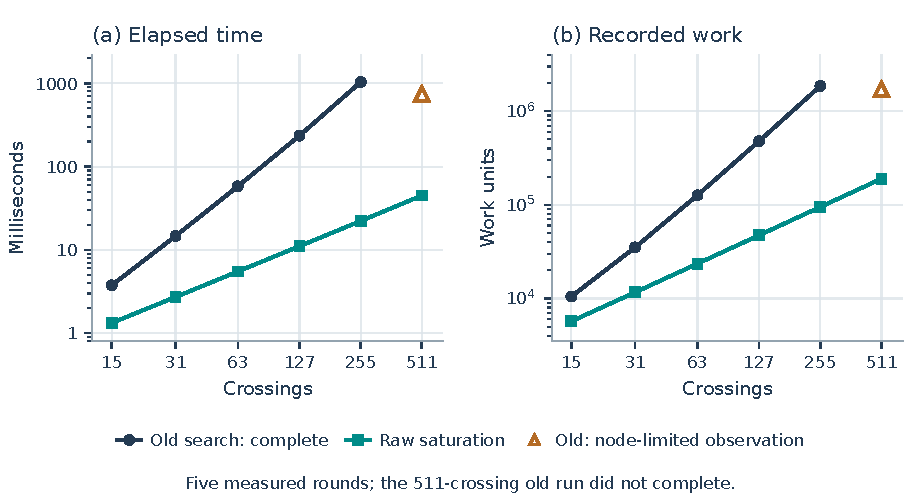
\includegraphics[width=\linewidth]{figures/raw_stage.pdf}
\caption{The complete group stage on elementary unknot closures.
Both source reconstruction and independent replay are included in
elapsed time. The marked old 511-crossing observation is node-censored.
These are mechanism controls, not a general hard-knot distribution.}
\label{fig:raw-stage}
\end{figure}

The maintained \texttt{unknot\_braid40} fixture improves from 22.536 to
3.387 ms in this isolated source-stage call, with paired ratio 6.625.
Other corpus cases show little benefit or regress. The paired ratios are
0.891 for \texttt{hard\_unknot\_8} and 0.912 for \texttt{monster}.
For \texttt{gordian}, the ratio is 1.010, too small to support a strong
elapsed-speed claim given the controls, and the exact work actually
increases. The source-stage benchmark cannot conclude knottedness when
group simplification fails: several nontrivial fixtures correctly remain
inconclusive in this positive-certificate stage.

\subsection{The failed-probe overhead and its correction}

The first candidate built a full support-incidence index before applying
the exact first-firing rejection test. On \texttt{gordian}, 137 of 139
queries failed this test, but 38,900 support incidences were nevertheless
materialized. The candidate used 986,374 work units against the
baseline's 789,805. Moving the guard before index construction reduces
this to 852,357, with only two indices and 32 materialized incidences.
The source audit confirms the same statuses and certificates as before.

This change removes most of the measured unnecessary index work, while
leaving an approximately 7.9\% work increase over baseline on this source.
The final work counts on \texttt{survivor-00} are 14,150 baseline versus
15,108 enabled; on \texttt{monster}, 5,357 versus 5,936. Both initial and
final records are supplied. It would be misleading to publish the large
algebraic-family speedup while omitting these failed-query costs.

\subsection{The surrounding recognizer changes the conclusion}

The full pipeline is tested on the 22 corpus fixtures with its normal
filters, a one-second total allowance, a 0.15-second local group
allowance, and the same remaining options for all arms. Every raw result
includes the terminal method and evidence, so an earlier filter's success
cannot be attributed to the new group producer. All conclusive outcomes
agree between arms. The full table is in
Appendix~\ref{app:full-tables}.

For example, \texttt{unknot\_braid40} is settled by the existing
genus-zero Seifert certificate before the group stage. Its full pipeline
times are about 0.21 ms in both arms, despite the large improvement when
the group stage is forced in isolation. The fixture \texttt{gst} is
rejected by the existing Alexander obstruction in about 1.3 ms, whereas
its positive-only group search stalls without a certificate. On
\texttt{gordian}, both pipelines reach the total time allowance and return
\texttt{UNKNOWN}; neither is credited with recognition.

For the survivor fixtures, enabled/full-pipeline paired ratios are mostly
slightly below one. The \texttt{monster} ratio is 0.903, corresponding
to medians 2.993 and 3.297 ms. Thus this corpus does not demonstrate a
broad improvement in full recognition speed. The new option remains
explicitly opt-in. Its supported benefit is complete raw reachability
and substantial improvement on some source-stage workloads, with the
observed regressions retained for future scheduling research.

\subsection{Orbit membership: independent graph audit and paired timings}

The eleven focused tests pass.  An exhaustive audit covers all systems with at most two interval generators
on universes of size at most five, up to input-generator order: $7{,}398$
indices across both merger rules and $34{,}026$ literal point checks.
The random audit prepares indices for $3{,}200$ random
interval relations under both maintained merger rules, giving $6{,}400$
checked indices and $208{,}000$ literal minimum comparisons.  A union-find
oracle explicitly expands only these bounded test inputs.  It also checks
$64{,}000$ sampled pair queries and all selected representatives, and all six
trace event types occur. The exhaustive and random tests also check the
complete canonical minimum interval set, sorted selection and ranks against
the literal graph. Two deliberately different valid traces establish
the distinction between canonical minimum labels and emission ordinals.

The geometric audit uses $67$ supplied normal vectors: parallel meridians
in one through ten tetrahedra and compatible mixtures of an interior
vertex sphere, a boundary vertex disc, and a one-sided M\"obius band in a
four-tetrahedron solid torus.  Both surface and boundary arc graphs are
tested under both merger rules, giving $268$ indices and another $73{,}528$
literal minimum comparisons.  These checks use the maintained exact
normal-coordinate adapter, with no native topology package required.
Separate tests cover $16{,}000$--$20{,}000$-bit endpoints, malformed and
unfinished proofs, source rebinding, caller mutation, disabled producer
entry points, and cancellation through false-valued callable objects.  A
separate exact fixture has $512$ disjoint minimum intervals and a $4{,}107$-bit
universe; its component count has $4{,}106$ bits, and the predicted $g=512$
interval bound is attained without enumerating components.

The portable paired benchmark has ten workloads, five shuffled arms,
one excluded warmup and seven measured rounds.  Single-query cases are
batched three times.  This gives $490$ measured complete arm calls and
$70$ warmup calls.  The compiled arm includes discovery, independent
verification, compilation and all requested comparisons.  The comparison
baseline shares the initial count and uses exact connected and singleton
shortcuts; only unresolved comparisons require augmented count schedules.
The original two-count API and identical controls are retained as separate
arms.  Every answer is compared outside the timer.

\begin{table}[htbp]
\centering
\caption{Complete repeated-membership workloads on supplied interval relations.
Discovery, independent verification, construction, and all queries are timed.
Times are milliseconds; ratios are paired medians.}
\label{tab:orbit-membership}
% Generated by generate_artifacts.py; edit the source JSON or generator.
\begingroup
\small
\setlength{\tabcolsep}{5pt}
\renewcommand{\arraystretch}{1.12}
\begin{tabular}{@{}p{6.5cm}rrrr@{}}
\toprule
Supplied relation & $q$ & Shared (ms) & Compiled (ms) & Ratio \\
\midrule
Meridian, $t=8$, scale $2^{512}+1$ & 1 & 2.845 & 2.993 & 0.925 \\
Meridian, $t=8$, scale $2^{512}+1$ & 8 & 12.880 & 2.852 & 4.582 \\
Meridian, $t=8$, scale $2^{512}+1$ & 32 & 46.957 & 2.996 & 15.629 \\
Meridian, $t=24$, scale $2^{128}+1$ & 1 & 25.157 & 20.437 & 1.224 \\
Meridian, $t=24$, scale $2^{128}+1$ & 8 & 111.298 & 20.308 & 5.502 \\
Meridian, $t=24$, scale $2^{128}+1$ & 32 & 422.509 & 20.539 & 20.686 \\
Primitive meridian, $t=8$ & 32 & 1.231 & 2.546 & 0.461 \\
M\"obius band, scale $2^{1024}+1$ & 32 & 1.540 & 0.321 & 4.447 \\
Four-tetrahedron compatible mixture & 32 & 29.527 & 2.124 & 13.915 \\
64-pair periodic chain & 32 & 14.182 & 1.629 & 8.757 \\
\bottomrule
\end{tabular}
\endgroup

\end{table}


\begin{figure}[htbp]
\centering
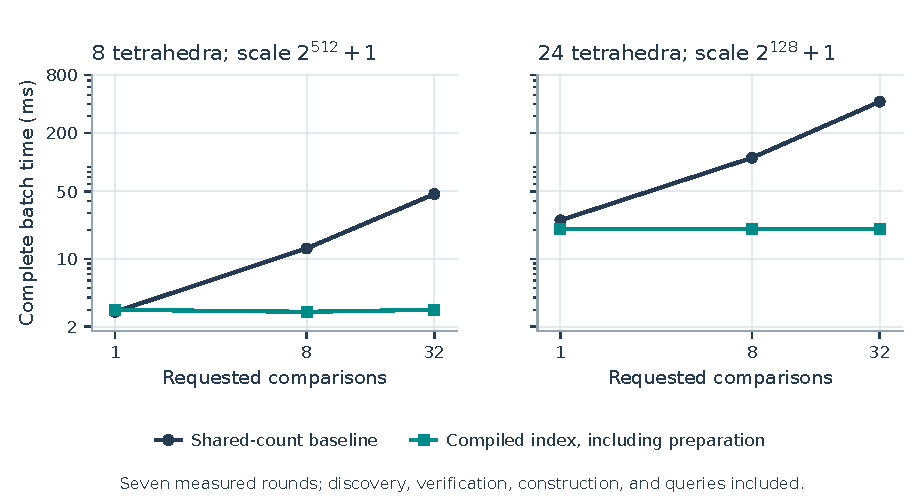
\includegraphics[width=\linewidth]{figures/orbit_queries.pdf}
\caption{Total membership-batch time as the number of requested comparisons
increases. Both compiled curves include preparation. No asymptotic law is
estimated from these finite observations.}
\label{fig:orbit-queries}
\end{figure}

Times are separate medians; the ratio is the median of paired ratios and
need not equal their quotient.  For the eight-tetrahedron source, the full
trace has $128$ events but the query program has $13$ point steps.  For
$24$ tetrahedra these figures are $832$ and $29$.  The periodic chain
compiles $65$ trace events to two point steps.  These are exact reductions
in work representation, independent of timer variation.

The primitive meridian is a necessary control: its first count proves the
relation connected, so the shared baseline answers all comparisons
immediately and is faster than index preparation.  The single-query
eight-tetrahedron case likewise shows no improvement.  Across all cases,
identical shared-control ratios range from $0.959$ to $1.040$, and
identical compiled-control ratios range from $0.969$ to $1.050$.  Thus the
large repeated-query effects are supported, while small percentage
differences should not be overinterpreted.

Raw records, inputs, query points, expected answers, reduction counts,
all shuffled arm orders and timings, and pre/post source hashes are in
\path{results/orbit_index.json}.  Audit evidence is in
\path{results/orbit_index_audit.json}; the portable drivers are in
\path{orbit_index_research/}.  Earlier prototype timings are not mixed into this table. Normal triangulation creation,
vector construction and conversion to interval relations are outside every
timer.  These results measure repeated queries on a supplied interval system,
not complete normal-surface calls or unknot-recognition runtime.
\subsection{Prepared canonical rank and selection}

The additional lookup experiment uses the sharp family of disjoint paired
blocks.  A supplied deterministic right-to-left trace is independently
verified before any query is timed.  The canonical minimum intervals and
every queried answer are checked against the direct block formulas, including
the conversion between emission ordinal and increasing-minimum rank.  Both
selection arms request the same original representatives on the same prepared
index; their numerical ordinal arguments differ because the orders differ.

Each measured call contains $512$ lookups, batched three times.  There are
seven shuffled measured rounds, one excluded warmup, and identical controls
for canonical rank and canonical selection.  Index construction is reported
separately and excluded from every lookup timer.  The original trace-ordinal
selection method reverses contractions; the canonical method searches the
compact minimum-interval union.

\begin{table}[htbp]
\centering
\caption{Prepared representative selection: 512 queries per call. Both selection
arms return the same source minima using their corresponding ordinals.
Preparation is excluded here and reported in the text. Times are milliseconds.}
\label{tab:orbit-rank}
% Generated by generate_artifacts.py; edit the source JSON or generator.
\begingroup
\small
\setlength{\tabcolsep}{5pt}
\renewcommand{\arraystretch}{1.12}
\begin{tabular}{@{}rrrrrr@{}}
\toprule
\shortstack{Minimum\\intervals} & \shortstack{Endpoint\\bits} & \shortstack{Emission\\(ms)} & \shortstack{Canonical\\(ms)} & Ratio & \shortstack{Rank\\(ms)} \\
\midrule
1 & 130 & 0.218 & 0.123 & 1.756 & 0.154 \\
16 & 134 & 0.794 & 0.138 & 5.922 & 0.168 \\
128 & 4105 & 7.600 & 0.327 & 23.791 & 0.348 \\
512 & 4107 & 29.732 & 0.365 & 81.511 & 0.408 \\
\bottomrule
\end{tabular}
\endgroup

\end{table}


All times concern a complete $512$-query call.  Preparation took respectively
$0.101$, $0.863$, $37.003$ and $557.962$ milliseconds in separately recorded
single observations.  Thus the submillisecond prepared lookup times do not
describe construction of the index.  Identical canonical-selection control
ratios range from $1.007$ to $1.034$, and rank-control ratios from $0.977$ to
$1.026$.  The final case has $512(2^{4096}+3)$ components while storing just
$512$ minimum intervals.  The bit-complexity conclusion is logarithmic in
the number of stored intervals, with binary-integer and output costs charged;
the finite timings are not a constant-time claim.

Full inputs, queried canonical ranks and corresponding emission ordinals,
analytic expected minima, source hashes, certificate hashes and all raw
samples are retained in \path{results/orbit_rank_select.json}.  The standalone
driver is \path{orbit_index_research/rank_select.py}.  This experiment measures
prepared representative lookups, separately from the preceding complete
membership-batch benchmark and from all unknot-recognition work.


\subsection{What these measurements support}

The strongest conclusions combine mathematical proofs with exact
representation or work counts: all raw orders reduce to a source closure
query; repeated component requests reuse one checked trace; minimum
representatives occupy at most the recorded number of static gaps.
Large local elapsed improvements are consistent with those mechanisms.
The same evidence rejects a claim that every diagram, every query count,
or the complete recognizer necessarily becomes faster.

The recent ReAPR study is relevant to the next empirical comparison:
its authors report success on a much larger public collection of unknot
diagrams, while treating general effectiveness as an open mathematical
question~\cite{reapr}. That study uses different methods and hardware.
We have not run its full corpus or its implementation here, so no
cross-paper speed ranking is made. A future complete-recognizer study
should include those inputs and comparable certified diagram
simplification strategies, alongside adversarial compressed presentations.
